\Chapter{Koncepció}
% TODO: Le kellene írni az OBJ formátumról a fontosabb dolgokat!
\Section{OBJ fájlformátum}

Az OBJ fájlformátumot elsőnek a Wavefront Technologies kezdte kifejleszteni az 1980-as években az Advanced Visualizer animációs csomagjához. Ez a formátum egy olyan karakteres fájlformátum, ami utat enged geometriai objektumok leírásának egy aránylag egyszerű és egységes formában.\cite{martinreddy}

Magát a formátumot ott logikus használni, ahol egyszerű modelleket jelenítünk meg és ezeket nem akarjuk animálni. Például egy olyan egyszerű autó szimulátoros játéknál, ahol maga az autó geometriáját tekintve nem változik maximum a pozíciója és az orientációja, ezeket a transzformációs mátrix állításával egyszerűen megadhatjuk, így nincs szükség a modell animálására.\\

\noindent Wavefront obj fájlformátum:\\

\noindent A formátum általános felépítése a kevetkezőképpen alakul:

Minden sor áll egy kezdő karakterből vagy szimbólumból, utána egy elválasztójel (szóköz vagy tabulátor). Rögtön ezután szám vagy szöveg következik.\\

\noindent Minden karakter, ami egy kettőskereszt (\#) karakter után helyezkedik el, az egy megjegyzés:

\bigskip
\begin{python}
# ez egy megjegyzes
\end{python}
\bigskip
Geometriai csúcsok:\\

\noindent \textbf{v} kezdőbetűvel ellátott sorok \textsl{geometriai csúcsot} definiálnak. Ezt követik (x, y, z [, w]) koordináták. A szögletes zárójel [ ] koordináta opcionális, alapértelmezés szerint 1.0 az értéke.
\bigskip
\begin{python} 
v -0,123 0,345 0,678 [1,0]
\end{python}
\newpage
\noindent Textúra koordináták:\\

\noindent \textbf{vt} kezdőbetűvel \textsl{textúra koordinátát} írunk le. Ezt (u, [, v, w]) koordináták követik, ezek 0 és 1 közötti értékek. A szögletes zárójel [ ] koordináta értékei opcionálisak és alapértelmezés szerint 0.0 az értékük.

\bigskip
\begin{python} 
vt 0.500 1 [0]
\end{python}
\bigskip
Normál csúcsok:\\

\noindent \textbf{vn} kezdőbetűs sorok \textsl{normál csúcsot} definiálnak. Ezt  (x, y, z) koordináták követik.
\bigskip
\begin{python} 
vn -0.500 0.500 -0.500
\end{python}
\bigskip
Lapelemek:\\

\noindent \textbf{f} kezdőbetűvel egy \textsl{lap elemet} írunk le. Az \textsl{lap elemet} \textsl{geometriai csúcs}, \textsl{textúra koordináta}, \textsl{normál csúcs} indexek listájával írjuk le {/} jellel elválasztva. Csúcs{\_}index {/} textura{\_}index {/}  normál{\_}index formátumban. Minden index 1-ről indul és növekszik annak sorrendjében, amelyben a hivatkozott elemet definiálták.\\

\noindent \textbf{Pár gyakran előforduló face definíció:}\\

\noindent Csak \textsl{geometriai csúcsokból} álló felület.
\bigskip
\begin{python} 
f v1 v2 v3 v4 ...
\end{python}
\bigskip
 Minden \textsl{geometriai csúcshoz} hozzá van rendelve egy \textsl{textúra koordináta} is.
\begin{python} 
f v1/vt1 v2/vt2 v3/vt3 ...
\end{python}
\bigskip
Minden \textsl{geometriai csúcs} tartalmaz \textsl{textúra koordinátát} és \textsl{normál csúcsot}.
\bigskip
\begin{python} 
f v1/vt1/vn1 v2/vt2/vn2 v3/vt3/vn3 ...
\end{python}
\bigskip
A \textsl{geometriai csúcshoz} csak a \textsl{normál csúcs} lett hozzárendelve, a \textsl{textúra koordináta} opcionális.
\bigskip
\begin{python} 
f v1/ /vn1 v2/ /vn2 v3/ /vn3 ...
\end{python}
\newpage
\noindentÖsszefoglalva, az OBJ formális nyelv kulcsszavakból (<\textbf{v}>, <\textbf{vt}>, <\textbf{vn}>, <\textbf{f}>), speciális karakterekből (<\textbf{/}>,<\textbf{\#}>) és számokból (<\textbf{Float}>, <\textbf{Integer}>) épül fel. Az OBJ nyelvtanát következő szabályokkal adhatjuk meg:\\

\noindent(OBJFájl) = {(Geometriai csúcs)}+{(Textúra koordináta)}+{(Normál csúcs)}+{(Lapelem)}\\
(Geometriai csúcs) = (v)+(Float)+(Float)+(Float)\\
(Textúra koordináta) = (vt)+(Float)+(Float)+[0]\\
(Normál csúcs) = (vn)+(Float)+(Float)+(Float)\\
(Lapelem) = (f)+{(Lap{\_}indexek)}\\
(Lap{\_}indexek) = (Integer)+[(/)+[(Integer)]+[(/)+[(Integer)]]]\\

\noindent A szögeltes zárójelbe [  ] foglalt elemek opcionálisak, vagyis a bennük lévő fogalom egyszer vagy egyszer sem jelenik meg a leírás során. \\

Wavefront formátum bemutatása példával, ez a példa egy szimpla négyszöget definiál:
\bigskip
\begin{python} 
v 0.0 0.0 0.0
v 1.0 0.0 0.0
v 1.0 1.0 0.0
v 0.0 1.0 0.0

vt 0.0 0.0
vt 1.0 0.0
vt 1.0 1.0
vt 0.0 1.0

vn 1.0 0.0 0.0 

f 1/1/1 2/2/1 3/3/1 4/4/1
\end{python}
\bigskip
A fájl először felsorolja a \textsl{geometriai csúcsokat} (\textbf{v}), utána a \textsl{textúra koordinátákat} (\textbf{vt}) és \textsl{normál csúcsokat} (\textbf{vn}), majd az \textsl{lap elemekkel} (\textbf{f}) egymáshoz rendeli ezeket. Ebben az esetben például a lapot négy csúcsponttal adtuk meg és {/} jellel elválasztva hozzá rendeltük a  \textsl{geometriai csúcsok} , a \textsl{textúra koordináták} és a \textsl{normál csúcsok} sorszámát.

A teljes OBJ formátum nagyon összetett, sok olyan szerkezeti egységet tartalmaz, ami egy szimpla objektum modellezéséhez szükségtelennek mondható.

\Section{Anyagjellemzők}

Az OBJ formátum 3D térben lévő objektumok csupán geometriáját írja le. Ezért szükségünk van még az anyagjellemzőkre is a képszintézis során. A különböző anyagokat fizikai jellemzőikkel írjuk le. Ezek a jellemzők például fényáteresztő képesség, fényvisszaverő képesség, törésmutató stb.\cite{diane1995mtl}\newpage
Ezeket a tulajdonságokat az MTL (Material Template Library) tartalmazza, a formátum hasonlóan az OBJ formátumhoz szintén szöveges. Az OBJ fájl tartalmazza a hivatkozást az {MTL} fájlra:
\bigskip
\begin{python}
mtllib fajlnev.mtl
\end{python}
\bigskip
Az \texttt{mtllib} hívja meg az MTL fájlt, ezután a \textsl{fájlnév} és a kiterjesztés következik \textsl{(.mtl)}.\\
OBJ fájlból akár egynél több anyagfájlra is lehet hivatkozni és egy MTL fájl tartalmazhat akár több anyagdefiníciót is.\\

\noindent A következő hívatkozással lehet beállítani a következő anyag anyagdefinícióját:
\bigskip
\begin{python}
usemtl (anyag neve)
\end{python}
\bigskip
Az anyag neve azonos egy anyagmeghatározással egy külső MTL fájlban.\\

\noindent Az objektumokat és sokszögcsoportokat a következő hivatkozások adják meg.
\bigskip
\begin{python}
o [objektum neve]
  ...
  g [csoport neve]
  ...
\end{python}
\bigskip
Sokszögek közötti árnyékolás a következővel állítható
\bigskip
\begin{python}
s 1
  ...
  s ki
  ...
\end{python}
\bigskip

\SubSection{MTL}
MTL fájl felépítése röviden:\\

Egy MTL ( Material Template Library) fájl tartalmazhat akár több anyagdefiníciót is. MTL fájl az anyagokat egymás után definiálja a fájlban, ezek a leírások \texttt{newmtl} paranccsal kezdődnek:
\bigskip
\begin{python}
newmtl szines
\end{python}
\bigskip
A \texttt{newmtl} egy új anyagot definiál, aminek a neve \texttt{"szines"}.
\newpage

\noindent A \textbf{Ka} kulcsszó az anyag ambient - környezettől független színét adja. Ez úgy viselkedik, mintha az anyag világítana, szóval ha a testet nem éri fény abban az esetben is ilyen lesz a színe. Viszont  az ambient tulajdonság nem viselkedik fényforrásként, attól hogy egy testnek ambient színe van az nem fogja megvilágítani a körülötte lévő többi testet. Az értéke RGB-ben van megadva 0 és 1 között.
\bigskip
\begin{python}
Ka 1.000 1.000 1.000
\end{python}
\bigskip
A \textbf{Kd} kulcsszó az anyag diffúz -  színét határozza meg. Ez a tulajdonság a test színét írja le, lényegében a diffúz tulajdonság meghatározza, egy felület rá eső fény mely részleteit nyeli el. Az értéke szintén RGB-ben van megadva 0 és 1 között.
\bigskip
\begin{python}
Kd 1.000 1.000 1.000
\end{python}
\bigskip
A \textbf{Ks} kulcsszó az anyag spekulár - színét adja. Ami az anyag tükröződéséért felelős. Értéke 0 és 1 között állítható. Amennyiben azt szeretnénk hogy az anyag minden ráeső fényt visszaverjen (tükörként működve), abban az esetben (1.0 1.0 1.0) értéket kell megadni ha pedig azt hogy mindet elnyeljen akkor (0.0 0.0 0.0) értékeket.
\bigskip
\begin{python}
Ks 1,000 1,000 1,000
\end{python}
\bigskip
Az \textbf{Ns} kulcsszó az anyag shininess - csillogását adja. Az anyagok felszíne nem csak tükörszerűen viselkedhetnek, hanem van saját fényük is. Ennek az értéke 0 és 1000 között határozható meg. Ezen skálán minél nagyobb értéket kap annál nagyobb lesz a fénysávok élessége.
\bigskip
\begin{python}
Ns 10.000
\end{python}
\bigskip
\Section{Textúrák}

Bár az OBJ fájl formátumnak nem része mégis fontos megemlíteni a textúrázást, a valóságszerű képek létrehozásánál egy fontos eszközünk a textúránk leképzése, hiszen a valóságban körülöttünk lévő tárgyak sem egyszínűek.

Textúrázás alatt általában kétdimenziós textúrázást értünk, de lehetnek ezek akár egy vagy háromdimenzionálisak is. A textúra geometriailag egy téglalap, ami sorokba és oszlopokba rendezet elemekből épül fel.

A textúra tehát adatok 1, 2 vagy 3 dimenziós tömbjének tekinthető. Az egyes textúra elemekhez tárolt adat képviselhet színt, fényerősséget vagy szín és alfa értékeket, azaz 1, 2, 3 vagy 4 adat  tartozhat minden textúra elemhez.

A téglalap alakú textúrákat azonban tetszőleges alakú sokszögekre, kell ráhelyezni. Ráhelyezést a modelltérben kell megadni, ezért  a textúráka is hatnak a modell- és vetítési transzformációk. Ennek érdekében az objektumok létrehozásakor a csúcspontok geometriai koordinátái mellett a textúra koordinátákat is meg kell adni, ezeknek a textúra koordinátáknak [0, 1] x [0, 1] egységnégyzeten belül kell elhelyezkedniük. \cite{juhasz2003opengl}
\Section{Modellbetöltő szofverek}

Manapság rengeteg modell elemző és betöltő szoftver áll rendelkezésünkre. A legtöbb ilyen szoftverről általánosságban elmondható, hogy ingyenes illetve  nyílt forráskóddal rendelkezik. Akadnak köztük elemzők online betöltők illetve telepítés után használható megjelenítők. Ezen szoftverek bemutatása következik.
\SubSection{Kixor modell elemző}

Az első ilyen elemző a Kixor modell elemzőszoftver volt.\cite{micah1987markup}\\
Elérési útvonal: \url{https://www.kixor.net/dev/objloader/}\\

A program futtatás után kielemezte a benne található \texttt{test.obj} fájlt \ref{fig:kixor}. ábra.
\bigskip
\begin{figure}[h]
\centering
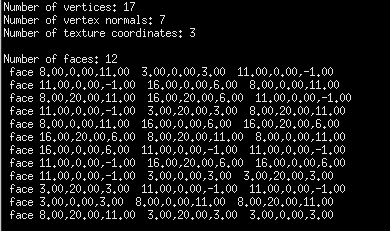
\includegraphics[scale=0.8]{images/kixor.png}
\caption{Kixor Elemző.}
\label{fig:kixor}
\end{figure}
\bigskip

\Aref{fig:kixor}. ábrán jól láthatóan módon a program elvégezte a szükséges számításokat majd visszatért a számított adatokkal.

Ez a szoftver nem alkalmas a modell megjelenítésére csak annak elemzésére viszont azt sok szemppontból megteszi, ha csak elemezni szeretnénk az OBJ fájlunkat abban az esetben kiváló lehetőségként szolgál.
\newpage
\SubSection{Online 3D Viewer}

Az első már megjelenítésre is alkalmas szoftver az Online 3D Viewer volt.\cite{online2014viktor}\\
Elérési útvonal: \url{https://3dviewer.net/}\\

Az oldalra érkezve \aref{fig:model_viewer1} ábran egy egyszerű és letisztult formátumot látunk, ahol rövid leírást ad a felhasználó számára, mik a támogatott fájlformátumok illetve azokat hogyan tudjuk megnyitni. 
\bigskip
\begin{figure}[h]
\centering
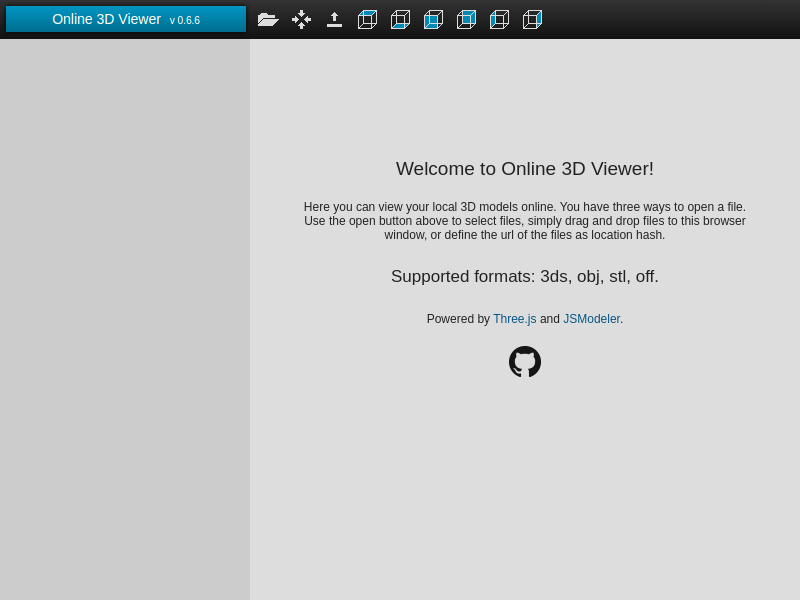
\includegraphics[width=\textwidth]{images/Model_Viewer.png}
\caption{Online 3D Viewer kezdőfelelület.}
\label{fig:model_viewer1}
\end{figure}
\bigskip

Mint \aref{fig:model_viewer1}. ábrán látható a számunkra lényeges \texttt{.obj} kiterjesztésű fájl formátum szintén a támogatott fájlformátumok között szerepel.

Leírásban benne van, hogy a megnyitás háromféleképpen történhet meg az oldal segitségével:
\begin{itemize}
\item Első lehetőségként az oldal bal felső részében található megnyitás gombra kattintva kiválasztjuk a megnyitni kivánt modellünket.
\item Második lehetőségként behúzzuk az oldalra a kívánt mdellünket egér segítségével.
\item Harmadik lehetőség pedig megadjuk a fájlok helyének webcímét.
\end{itemize}
\newpage
Miután kiválasztottuk a megfelelő objektumot az automatikusan megjelenik a rajzfelületen \aref{fig:model_viewer2} ábra.
\bigskip
\begin{figure}[h]
\centering
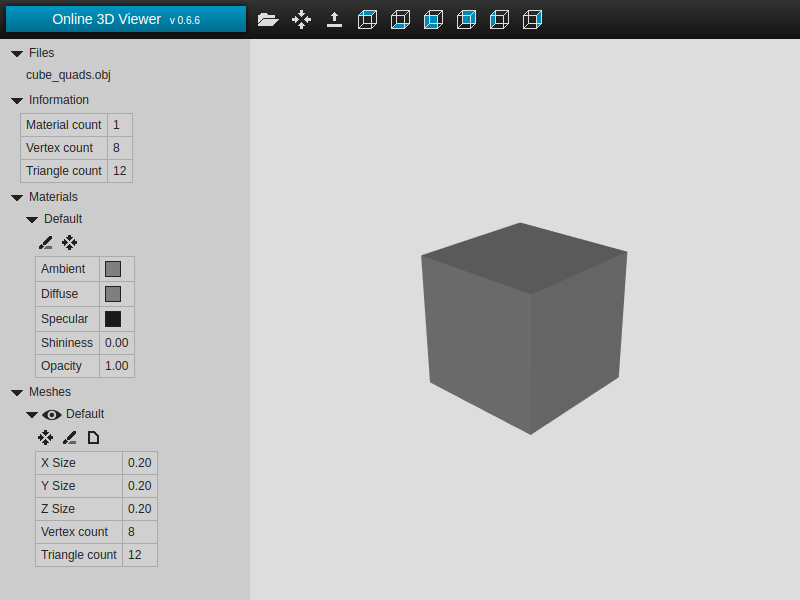
\includegraphics[width=\textwidth]{images/Model_Viewer_2.png}
\caption{Online 3D Viewer modell betöltéssel.}
\label{fig:model_viewer2}
\end{figure}
\bigskip

Rajzfelülettől balra találhatóak az objektumunkról gyűjtött adatok. Felette a model egyes síkidomjainak központba helyezése, a modellünk forgatása bal egérgomb folytonos nyomva tartásával és egér mozgatásával történhet. Ezen felül kameránk közelítése és távolítása görgő segítségével kivitelezhető.

A modellbetöltő gyors és egyszerű megjelenítést biztosít számunkra, tökéletesen működik a bonyolultabb geometriájú síkodomok megjelenítésével legyen szó háromszög, négyszög vagy akár ennél nagyobb csúcsszámmal rendelkező síkodomról. Ez nagy előnyt jelent felhasználó szempontból, amennyiben csak a modell megjelenítése a cél.

Sajnos kép alapú textúrázás nem támogatott a program által, ezért a textúrázás nem lehetséges. Másik probléma a szoftverrel, hogy egy időben csak egy OBJ file kirajzolására alkalmas.\\

Betöltő forráskódja illetve a programmal kapcsolatos rövid leírás megtalálható a következő weboldalon:

\url{https://github.com/kovacsv/Online3DViewer}
\newpage
\SubSection{Creators 3D Online Viewer}

Másik ilyen internetes betöltő a Creators 3D Online Viewer.\cite{creators2018creators3d}\\
Elérési útvonal: \url{https://www.creators3d.com/online-viewer}\\

\noindent Hasonlóan az előző Online 3D Viewer-hez a betöltő kezdőfelületén \aref{fig:3d1} ábra szintén tájékoztatást ad a támogatott fájlformátumokról.

Ez a betöltő is támogatja a OBJ fájl megjelenítését. A betöltő szintén támogatást nyújt a különböző sokaságú csúcspontal rendelkező síkidomok betöltésével, az előzőtől eltérően itt a megnyitás kétféle képpen történhet

\begin{itemize}
\item Első lehetőség: \\
A rajzfelültre húzzuk a megjelenítésre szánt objektum fájlunkat .
\item Második lehetőség:\\
Rajzfelületre kattintva megadjuk a fájlunk lokális helyének az útvonalát.\\
\bigskip
\begin{figure}[h]
\centering
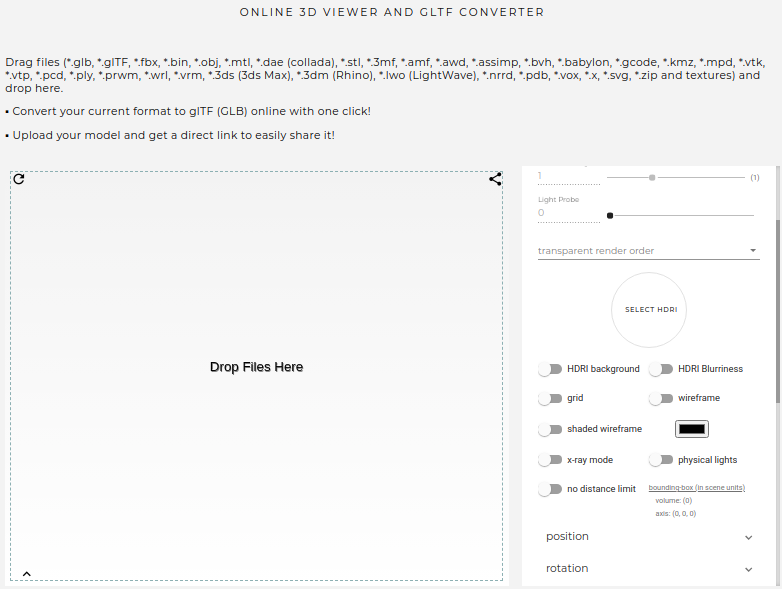
\includegraphics[width=\textwidth]{images/3D_creators.png}
\caption{Online 3D Viewer kezdőfelület.}
\label{fig:3d1}
\end{figure}
\bigskip

Rajzfelületre kattintva megadjuk a fájlunk lokális helyének az útvonalát.\\
\end{itemize}
\newpage
\bigskip
Amint kiválasztjuk a megjelenítésre szánt fájlunkat a felsorolt két lehetőség közül az objektum megjelenik a rajzfelületen \aref{fig:3d2}. ábra.
\bigskip
\begin{figure}[h]
\centering
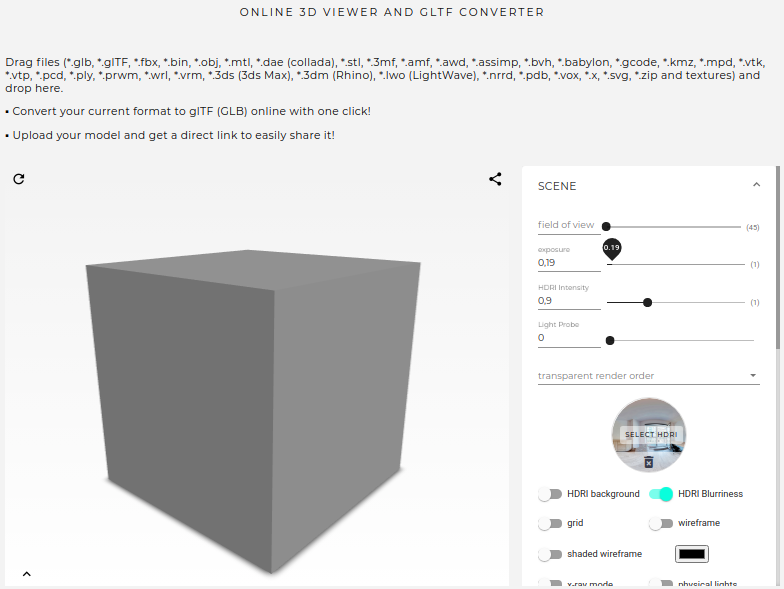
\includegraphics[width=\textwidth]{images/3D_creators_2.png}
\caption{Online 3D Viewer modell betöltéssel.}
\label{fig:3d2}
\end{figure}
\bigskip

Előző betöltőhöz hasonlóan szintén nagyon gyorsan megjelenítette a betöltésre szánt modellünket. Nyilván minél komplexebb a modellünk annál arányosabban több időbe telik a betöltés.

\newpage
Rajzfelülettől jobbra találhatóak különböző beállítások a megjelenítéssel kapcsolatban. Ilyenek például a keret kirajzolása (wireframe), aminek bekapcsolásával csak a modell hálója látszódik a \ref{fig:3d3}. ábrán.
\begin{figure}[h]
\bigskip
\centering
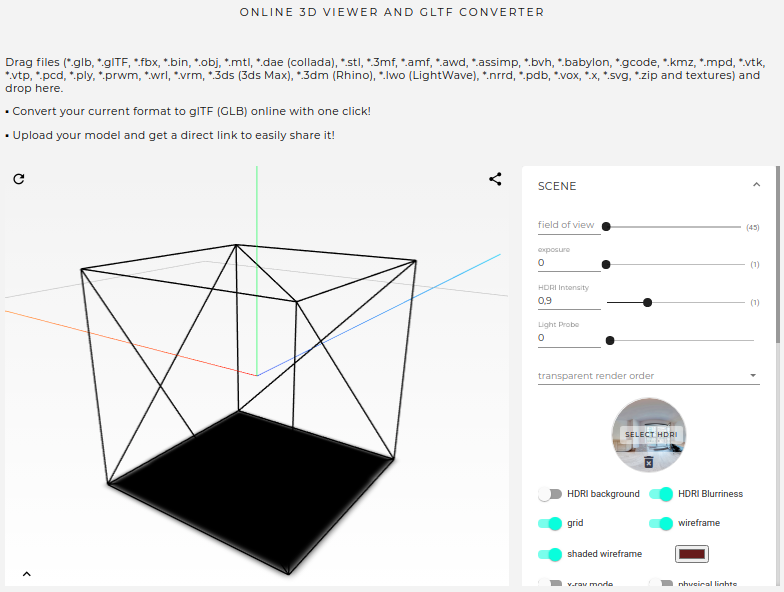
\includegraphics[width=\textwidth]{images/3D_creators_4.png}
\caption{Online 3D Viewer keret kirajzolással.}
\label{fig:3d3}
\end{figure}
\bigskip

De sok más egyéb funkcióval is ellátott például megjeleníthető koordináta tengely (grid), aminek segítségével vizsgálhatjuk az objektumunk irányultságát illetve elhelyeszkedését az x, y tengely kék és piros vonallal lettek jelezve a z tengely pedig zöldel  \ref{fig:3d3}. ábra.
\newpage
\SubSection{Model Loader}
Következő tesztelt szoftver, a Piller Imre által fejlesztett Model Loader volt.\cite{imre2020model}\\

\noindent A betöltő szoftverről részletes magyar nyelvű leírás és használati útmutató a következő webcímen található: \url{https://www.uni-miskolc.hu/~matip/grafika/}\\

A weboldalon található teljes dokumentáció beleértve : fejlesztő környezet beüzemelése, egyszerű objektumok kirajzolás, anyagjellemzők beállítása illetve textúrázás.

Ez a betöltő támogatja a kép alapú textúrázást, több objektum egy időben való betöltését  ezeket akár különböző textúrával illetve anyagjellemzővel is megjeleníthetjük.\\

Fejlesztői környezet beállítása után első futtatásra a \texttt{cube.obj} nevű példa a hozzátartozó textúrával következőképpen néz ki betöltés után (\ref{fig:model1}. ábra).
\bigskip
\begin{figure}[h]
\centering
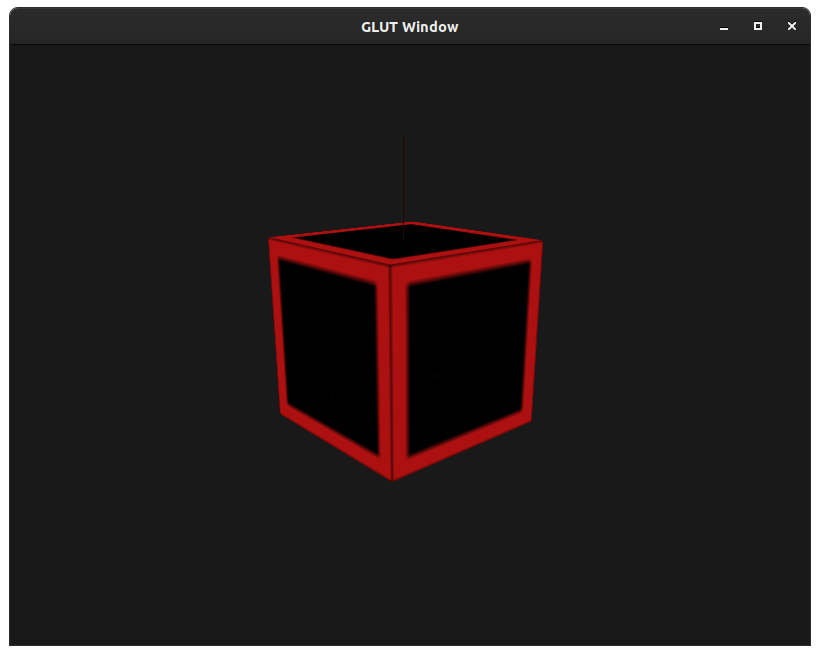
\includegraphics[width=\textwidth]{images/Model_loader.png}
\caption{Cube.obj megjelenítése.}
\label{fig:model1}
\end{figure}
\bigskip

Megjelenítés teljesen jól történt a megjelenítendő objektumot egy külön ablakban kirajzolta a program. A textúra illesztésével nem volt gond.\\
\newpage
Majd különböző komplexitású modellek betöltését teszteltem \ref{fig:modelbaby}. és  \ref{fig:modelbird}. ábrák.
\bigskip
\begin{figure}[h]
\centering
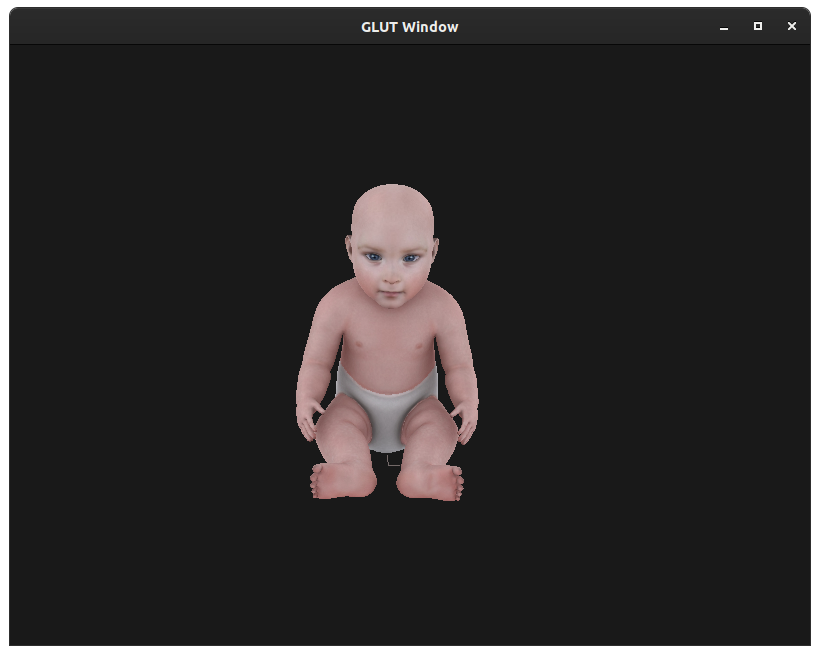
\includegraphics[scale=0.35]{images/model1.png}
\caption{Baby.obj modell megjelenítése.}
\label{fig:modelbaby}
\end{figure}
\bigskip
\begin{figure}[h]
\centering
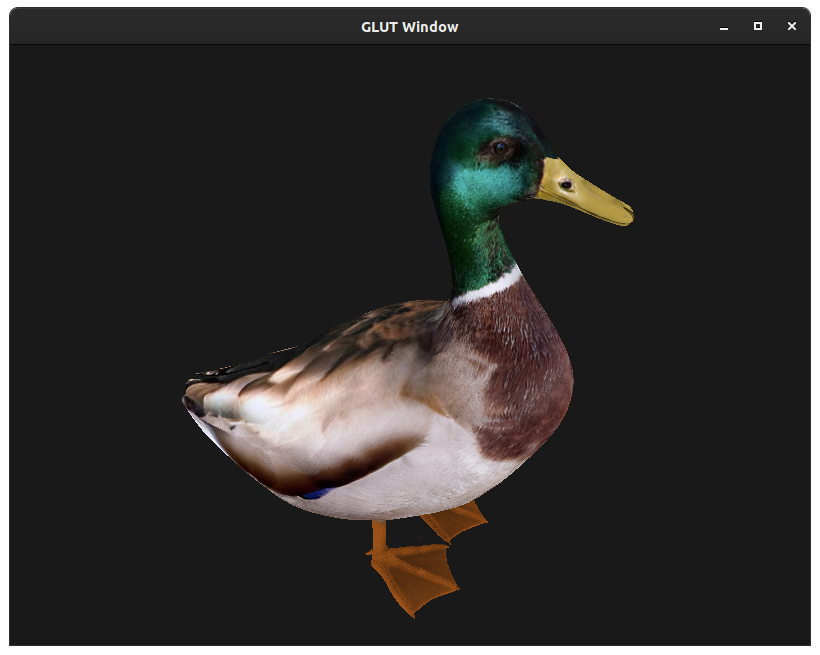
\includegraphics[scale=0.35]{images/bird.png}
\caption{Bird.obj modell megjelenítése.}
\label{fig:modelbird}
\end{figure}
\bigskip

Ezek a modellek szintén tökéletes megjelenítésre kerültek, a hozzájuk tartozó textúra betöltésével nem volt gond a modell megjelent a rajzfelületen.
\newpage
Pár ilyen betöltés után észrevettem,hogy a betöltő nem kezel háromszögnél nagyobb csúcspontal rendelkező síkidomokat,  \aref{fig:model1} ábra megjelenített \texttt{cube.obj} háromszögeit át konvertáltam négyszögekké, majd ezek után szintén betöltöttem a megjelenítőbe (betöltés \ref{fig:model2} ábra).
\bigskip
\begin{figure}[h]
\centering
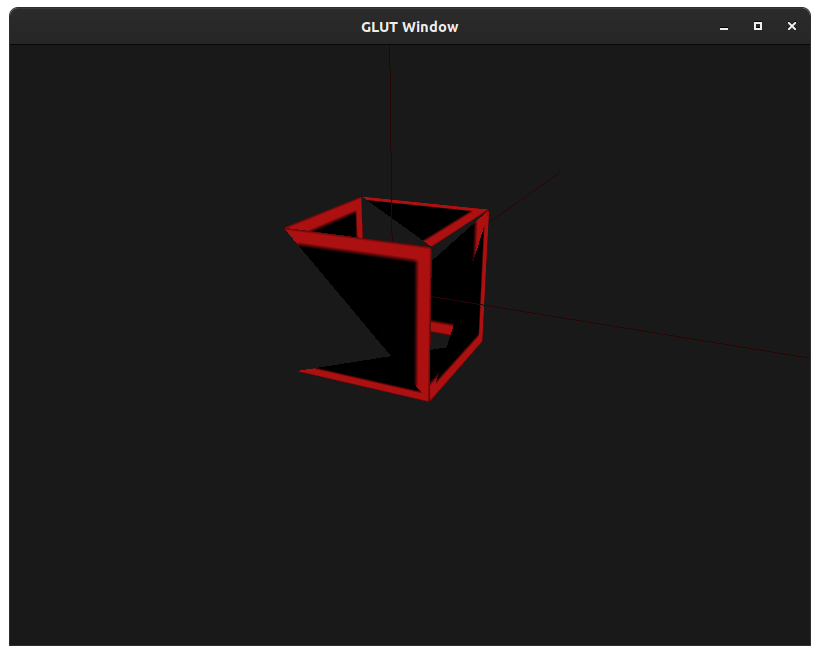
\includegraphics[width=\textwidth]{images/Model_quads.png}
\caption{Cube Model négyszögekkel.}
\label{fig:model2}
\end{figure}
\bigskip

Az ábrán jól látható hogy az objektum megjelent az ablakban viszont a kirajzolás nem megfelelő módon történt a kockánk eléggé hiányos, hiányzik a síkidomokról a negyedik csúcspont. A javító programunk egyik tervezett része ennek a hibának a javítására szolgál.
%\Section{Obj fájl formátum}
%\Section{Obj elemző szoftverek}
%\Section{Obj Bickbucket}
%\Section{Obj Bickbucket teszt}